% Whisker barrel generation paper equations, for pasting into Google
% docs draft.

% While writing, don't stop for errors
%\nonstopmode

\documentclass[a4paper,11pt]{article}
\usepackage{amsmath,amssymb,mathtools}
\usepackage{enumerate}
\usepackage{times}
\usepackage[usenames]{color}
\usepackage{parskip}
\usepackage{afterpage}
\usepackage{setspace}
\usepackage[modulo]{lineno}
%\usepackage{xltxtra}
%\usepackage{xunicode}
\usepackage{gensymb}

\usepackage{titlesec}
\titleformat*{\section}{\LARGE\bfseries}
\titleformat*{\subsection}{\Large\bfseries}
\titleformat*{\subsubsection}{\large\bfseries}
\titleformat*{\paragraph}{\large\bfseries}
\titleformat*{\subparagraph}{\large\bfseries}


\setcounter{tocdepth}{3}
\usepackage{graphicx}
\usepackage{comment}
\usepackage{textcomp}
\usepackage{natbib}

\usepackage{lmodern}

\usepackage[labelfont=bf,labelsep=period,justification=justified]{caption}

\doublespacing
\topmargin 0.0cm
\oddsidemargin 0.5cm
\evensidemargin 0.5cm
\textwidth 16cm
\textheight 21cm
\makeatletter
\makeatother
\date{}
\pagestyle{plain}

% Blue for comments
\newcommand{\cmnt}[1]{\textcolor{blue}{#1}}
% Code in sans serif
\newcommand{\code}[1]{\textsf{#1}}
% Divergence symbol (Del dot Del)
\newcommand{\dvrg}{\nabla\vcdot\nabla}
% Emphasis shortcut
\newcommand{\e}{\emph}
% Bold shortcut
\newcommand{\bol}{\textbf}
% Math bold
\newcommand{\mb}[1]{\mathbf{#1}}
\makeatletter
\newcommand*\vcdot{\mathpalette\vcdot@{.35}}
\newcommand*\vcdot@[2]{\mathbin{\vcenter{\hbox{\scalebox{#2}{$\m@th#1\bullet$}}}}}
\makeatother

%\bibliographystyle{plos2015}
\bibliographystyle{apalike}


\begin{document}
%\begin{center}
\begin{flushleft}
{\huge
\textbf{Self-organization of whisker barrels in simulation requires competition between thalamocortical axons}
 \vspace{5em}
}
%\end{center}

Sebastian~S.~James$^{1*}$, Stuart~P.~Wilson$^{1}$ \vspace{1em}\\
$^{1}$Department of Psychology, The University of Sheffield, Sheffield, United Kingdom.\vspace{1em}\\
$^{*}$Corresponding author email: Seb.James@Sheffield.ac.uk\vspace{1em}\\
Short title: Self-organising whisker barrels\vspace{5em}\\
\end{flushleft}

\newpage{}
%\raggedright

\section*{Abstract}

Understanding how genetic information and spontaneous pattern formation
together give rise to the whisker barrels is an important challenge for
developmental neurobiology. The barrel patterning that coalesces in layer IV
has been described formally as a Voronoi tesselation, which is indicative of
an underlying developmental process based on local competitive
interactions. If pattern formation relies only on such intrinsic
self-organising processes, how can the somatotopic order at the periphery be
maintained in the projections from brainstem to thalamus and from thalamus to
cortex? To investigate, we began by extending a computational model of
neocortical arealization by Karbowski \& Ermentrout (2004; J. Comp. Neurosci.)
to generate fields on a two-dimensional cortical sheet. Central to this model
is an assumption that axonal branching and synaptogenesis are coupled, and
that thalamic projections compete for cortical territory under the influence
of molecular signalling gradients. We found that these processes alone are
incapable of generating patterns of cortical fields that are more intricate
than the patterns already present in molecular guidance signals. However, a
full barrel-field pattern emerges under the guidance of as few as four
signalling gradients when the model is extended to introduce competition
between the branches of axons that originate from different thalamic
barreloids. We show that the key requirements for the emergence of realistic
(Voronoi tesselation) patterning are i) at each cortical location
thalamocortical projections compete for a limited number of available
connections, ii) at each location the axonal branching rate of each
thalamocortical projection is reduced by the total branching density of the
other projections, and iii) the density of axon branching for each
thalamocortical projection is conserved. We demonstrate how a purely
self-organising system can initialise a pattern which can then be faithfully
replicated in multiple neural structures. We show that this minimal model of
barrel self-organisation provides a parsimonious account of data from a range
of classic studies in which intrinsic and extrinsic factors have been
experimentally manipulated.


\section*{Introduction}

\modulolinenumbers{}
\linenumbers

Spatial patterns in neural connectivity provide clues about the constraints
under which brains evolve and develop. Whether or not patterning governs
information processing, models of the development of information processing
circuits can be validated in terms of their ability to account for biological
patterning (\citealp{purves_iterated_1992}; see also
\citealp{wilson_what_2015,bednar_cortical_2016}). One of the most distinctive patterns of
neural connectivity is found in the rodent barrel cortex
(\citealp{woolsey_pattern_1948,woolsey_structural_1970,welker_structure_1974}, see
\citealp{fox_barrel_2008}). Understanding how this particular pattern forms might shed
light on the interplay of genetic and extrinsic factors that shape cortical
circuits, and on a wealth of anatomical, physiological, and behavioural data
obtained using this model system.

The barrels are large cortical columns, identifiable from birth in layer 4 of
rodent primary somatosensory cortex as dense clusters of thalamocortical
axons, which are enclosed by borders a few neurons thick from postnatal day 3
\citep{erzurumlu_development_2012}. In the plane tangential to the cortical surface the
barrels constitute a map of the arrangement of the whiskers on the
face (see \citealp{yamakado_subdivision_1979}), such
that the cells of adjacent barrels respond most strongly and most quickly to
deflection of adjacent whiskers \citep{armstrong-james_flow_1992}. The barrels
reflect subcortical whisker maps comprising cellular aggregates known as
barrelettes in the brainstem and barreloids in the thalamus
\citep{killackey_pattern_1980}.

Each whisker and its corresponding barrelette, barreloid, and barrel can be
identified by its position on a two-dimensional grid
\citep{zucker_coding_1969,killackey_pattern_1980,van_der_loos_barreloids_1976,haidarliu_size_2001}. The barrels are normally up to
twice as long in the axis aligned to the grid ‘rows’ compared to the ‘arcs’,
and the rows are visible from day 2 \citep{rebsam_refinement_2002} whereas the arcs become
distinct by day 3 \citep{erzurumlu_development_2012,rebsam_refinement_2002}. In metabotropic glutamate
receptor 5 (mGlu5) knockouts the barrel rows develop but the arcs do not
(\citealp{hannan_plc-1_2001} see also \citealp{fox_barrel_2008}), thus distinct processes
likely guide development of the barrels with respect to the orthogonal grid
axes.

Barrel formation requires afferent input, driven by whisker stimulation and by
thalamic calcium waves that propagate via mGlu5-receptor activation
(\citealp{anton-bolanos_prenatal_2019}, see also \citealp{anton-bolanos_developmental_2018}). Patterning also depends
on a complex network of axon guidance processes, which includes interactions
between guidance molecules like ephrin-A5 and A7 \citep{miller_epha7-ephrin-a5_2006} and
between adhesion molecules like cadherin-6 and 8 \citep{greig_molecular_2013,bishop_regulation_2000},
and the binding of p75 to neurotropins (\citealp{shimogori_fibroblast_2005,bishop_distinct_2002};
see also \citealp{dye_lifespan_2011,dye_lifespan_2011-1}). This network is orchestrated by
interactions between morphogens Fgf8 and Fgf17 and transcription factors Emx2,
Pax6, Sp8, and Coup-tf1 \citep{shimogori_fibroblast_2005,bishop_regulation_2000}, which are expressed
in gradients that mark orthogonal axes and can be manipulated to cause the
barrels to stretch, shrink, shift, skew, and even duplicate
\citep{shimogori_fibroblast_2005,assimacopoulos_fibroblast_2012,borello_sp8_2014,sahara_sp8_2007,ypsilanti_transcriptional_2016,sur_patterning_2005}.

The boundaries of the barrels form polygonal shapes that together
create a Voronoi tesselation across the cortical sheet, wherein all
points enclosed by a given boundary are closer to its center than to
the center of any other boundary \citep{senft_mouse_1991}. This
patterning suggests that the barrel topology may be preserved in the
initial projection of the thalamocortical axons into the cortex, and
that a barrel forms by the lateral branching of the axons from their
initial centres of mass, which ceases upon contact with the axons
branching from adjacent centres. According to this model the barrel
pattern could be entirely determined by the distribution of the
initial centre points, which would itself be determined by guidance
cues. However, the assumption of pre-arranged centres is difficult to
resolve with the observation that thalamocortical axons arrive in the
cortical plate as an undifferentiated bundle prior to barreloid
formation (\citealp{agmon_organized_1993}; see \citealp{erzurumlu_development_2012} for a review).

Alternatively, reaction-diffusion dynamics could generate a Voronoi-like
tesselation in the cortex without the need for pre-arranged centres, by
amplifying characteristic modes in the noisy initial distribution of bundled
axon branches, as a net effect of short-range cooperative and longer-range
competitive interactions between cells. According to this model the barrel
pattern would be determined by the relative strength of these interactions and
by the shape of the cortical field boundary. However, reaction-diffusion
dynamics alone are unlikely to be able to account for the precise
co-registration and topographic connectivity between emergent domains in
thalamus and cortex, the non-uniform sizes and spacing of the barrels to form
rows versus arcs, and the influence of gene expression gradients.

As theories of barrel patterning, the centre-point and reaction-diffusion
models are not mutually exclusive. Pre-organised centres in the initial
conditions could bias reaction-diffusion processes to generate the specific
somatotopic arrangement of barrels more reliably, and similarly the mechanisms
by which axons branch laterally from barrel centres may involve a tension
between cooperative and competitive interactions. However, a proof that barrel
patterning can in principle emerge within an undifferentiated bundle of
thalamocortical axons, based only on local interactions between cells, would
remove the need to invoke a global supervisor, i.e., to assume a separate
stage and/or extrinsic mechanism for pre-organising thalamocortical
connections.

To this end, the aim of the present study is to establish whether it is
possible for the observed arrangement of barrels to self-organise in a system
governed by reaction-diffusion dynamics, under the guidance of molecular
signalling gradients, and in the absence of pre-defined centre-points. Our
approach is to represent in a computational model the minimal set of
biological assumptions that might lead to the emergence of barrel patterning
in simulation, and, if necessary, to add to this minimal set only assumptions
that can be represented by the local exchange of information between adjacent
cells. The emergence of barrel patterning under such conditions would serve as
an existence proof of the plausibility of the hypothesis that barrel
development is a self-organising process.

\section*{Models}

\cite{karbowski_model_2004} developed what remains, to the best of our knowledge, the
only dynamical model of cortical arealization capable of generating
predictions about the influence of signalling molecules on the size, shape,
and topological organization of emergent cortical fields. This model describes
competition between thalamocortical projections for territory along a
one-dimensional string of cortical cells, e.g., along an anterior-posterior
axis. The equations of the model define how the density of connections, $c$,
and the density of axon branches, $a$, interact at time $t$ at each cortical
location $x$, for $N$ thalamocortical projections indexed by $i$. The Voronoi
tesselation used to describe barrel patterning is a two-dimensional structure,
hence we first extended the original model for simulation on a two-dimensional
cortical sheet, and describe it here as such (i.e., substituting $x$ with the
two-dimensional position vector $\mb{x}$ and substituting terms of the form
$\frac{d}{dx}$ with the spatial gradient operator $\nabla$).

The original model was derived from the assumption that the rates at which
thalamocortical synapses form and thalamocortical axons branch are
reciprocally coupled, resulting in an expression for the change in $c_i$ as a
function of $a_i$, and for the change in $a_i$ as a function of
$c_i$. Synaptogenesis is modelled as

\begin{equation} \label{eq:dc}
\frac{\partial c_i(\mb{x},t)}{\partial t} =-\alpha c_i(\mb{x},t) +\beta  \left(1 - \sum_{i'=1}^{N} c_{i'}(\mb{x}, t)\right)[a_i(\mb{x},t)]^k.
\end{equation}

Accordingly, when the final term evaluates to zero, the density of
thalamocortical connections decays exponentially at a rate given by the decay
constant $\alpha$. This occurs where the density of connections over all
thalamic projections sum to one; interpreted as a state in which all of the
available synaptic receptors within the cortical dendritic trees are
occupied. Otherwise, the connection density is assumed to vary non-linearly
($k>1$) with the axon branching density.

Changes in axon branching density are assumed to depend also on the
influence of guidance molecules and on the density of branches at
adjacent cortical locations:

%
\begin{equation} \label{eq:da}
\frac{\partial a_i(\mb{x},t)}{\partial t} = \nabla\vcdot\left(D \nabla a_i(\mb{x},t)-a_i(\mb{x},t)\sum_{j=1}^{M} \gamma_{i,j}\nabla \rho_j(\mb{x})\right) - \frac{\partial c_i(\mb{x},t)}{\partial t} + \chi.
\end{equation}

The first term on the right describes the divergence (indicated by
$\nabla\vcdot$) of a quantity referred to in models of heat diffusion as the
`flux' (the term enclosed by parentheses). The central idea in heat diffusion
models is that the change in temperature (over time) at a given location is
proportional to the gradient in the temperature (over space) at that
location. Substituting the branching density for heat, axons from a given
thalamic projection are thus assumed to branch laterally across the cortical
sheet at a rate given by the diffusion constant $D$. Lateral branching is
augmented by a measure of the local alignment between the branching density
and the gradient in the concentration of each of $M$ distinct molecular
signals, $\rho(\mb{x})$. The influence of a given signal (indexed by $j$) on a
given thalamic projection (indexed by $i$), is determined by the parameter
$\gamma_{i,j}$. Interactions for which this value is positive encourage axon
branching in the direction in which the concentration of the signal is
increasing, whereas negative interactions encourage branching in the opposite
direction. Hence the axons of a given thalamic projection are assumed to
branch towards either higher or lower concentrations of each signalling
molecule.

The second term on the right of equation 2 represents an assumption that the
axon branching density decreases when the number of connections being made
increases, and vice versa, i.e., that branches are required to form synaptic
connections. Note that we introduce the term $\chi=0$ here, so that we might
subsequently redefine $\chi$ to introduce the competition between thalamic
projections that we will show to be necessary for the emergence of a Voronoi
tesselation (see Results).

Two points are important to emphasise here. First, notice that the only
difference between thalamic projections is the interaction strengths,
$\gamma$. Hence any differences between the size, shape, and location of
cortical fields that reliably emerge from the dynamics of the model must be
due to differences in the choice of these values only. Second, the formulation
of the model is at this point entirely local, in the sense that simulating the
dynamics requires no information to be communicated from cortical locations to
any but the immediately adjacent locations.

In addition to the choice of initial conditions (for the fields
$c(\mb{x},t=0)$ and $a(\mb{x},t=0)$) and the axon guidance fields
$\rho(\mb{x})$, the free parameters of the model are the number of
thalamocortical projections, $N$, constants $\alpha$, $\beta$, $k$, and $D$,
and the $N\times M$ interaction strengths, $\gamma$.

The dynamics of the model (equations 1 and 2) were solved on a hexagonal
lattice of grid elements representing the cortical sheet, under the assumption
that axon branches cannot extend beyond the boundary of the sheet, i.e.,
$\mb{J}_i(\mb{x},t) \bigg\rvert_{boundary} = 0$. We developed software tools
for imposing arbitrary boundary shapes, specified in a scalable vector
graphics (.svg) file format, on the lattice. The dynamics were numerically
integrated using fourth-order Runge-Kutta, and using a {\color{red} finite
  difference method} to compute the flux term (see Supplementary Materials).

\section*{Results}

%\cmnt{If we need to present the results of the 2-D system with $\chi=0$, then
%  we'll do that first, showing a 2-D version of the simulation obtained by
%  running \code{james0 configs/karb.json}}

We first verified that the system given by Eqs.~\ref{eq:dc} \& \ref{eq:da}
described a two dimensional extension of the axon branching model in
\citet{karbowski_model_2004}. We showed that in the presence of three guidance
gradients varying only in one dimension (along the long axis of an elliptical
domain), five thalamocortical axon types, each interacting uniquely with the
three guidance gradients, would segregate into five separate regions. We
investigated a number of configurations of the guidance gradients, varying
their shape, $\rho(\mb{x})$, and number, $M$, and their effect on a varying
number of thalamocortical projections, $N$. In general, we were not able to
producen a complexity of structure in the resulting patterns of the
connections, $c(\mb{x},t\rightarrow\infty)$, which was not present in the
guidance patterns.

Complex structure can indeed be observed in protein expression for some genes,
such as the molecules Bhlhb5 \citep{joshi_bhlhb5_2008} and Lmo4
\citep{cederquist_lmo4_2013,greig_molecular_2013}. These expression patterns
can therefore provide a theoretical mechanism for the guidance of axons into
distinct regions.
%The question of how such structures are generated becomes
%one of of how gene transcriptional interactions and mRNA diffusion and
%movement achieves this (\cmnt{Fixme: find a ref on structure in gene
%  transcription}).
However, complex and stable structure in gene expression data is not commonly
reported; monotonically varying expression patterns, such as those for Pax6,
Emx2 \citep{shimogori_fibroblast_2005,bishop_regulation_2000},
Sp8~\citep{sahara_sp8_2007} and Coup-tf1~\citep{borello_sp8_2014}, which
display graded expression across the entire isocortex are more
typical. Furthermore, the complex structure observed in the whisker barrel
field has not, to our knowledge, been linked to a set of gene expression
patterns matching the scale of the barrels. To investigate how the whisker
barrel structure might form in the presence of only monotonically varying
morphogen gradients, we turned our attention to the competition for
connections built into the model.


\subsection*{Branching competition is required to form somatotopically ordered barrels}

There exists an element of competition in the model system specified by
Eqs.~\ref{eq:dc} \& \ref{eq:da}. The term $\left(1 - \sum_{i=1}^{N}
c_i(\mb{x}, t)\right)$ in Eq.~\ref{eq:dc} ensures that once the available
synaptic receptors in a region have been fully occupied, say by
thalamocortical type $i=1$, there is no longer the possibility for type $i=2$
to form any synapses. This competition turns out to be relatively weak,
because it does not strongly affect the branching density in that region. In
the model, it is possible for two or more TC axon types to have roughly equal
branching density in some region, leading to roughly equal numbers of
connections forming for each TC type, up until the `hard' connection limit
is reached.

To introduce competition between the \emph{branching} of thalamocortical axon
types, we introduced the new term $\chi$ given by
%
\begin{equation} \label{eq:branch_comp}
\chi(\mb{x}, t) = - \frac{\epsilon  a_i(\mb{x}, t)}{N-1} \sum_{i' \ne i}^{N} a_{i'}(\mb{x}, t).
\end{equation}
%
which leads to a reduction in the rate of increase of branching density for
axon type $i$ in regions where the branching density of \e{other} axon types
is high.

This introduces a new parameter, $\epsilon$, which governs the strength of the
branching competition. The factor $1/(N-1)$ ensures that the branching
competition strength scales with the number of TC axon types in the system.

With the addition of the competition term, $\chi$, it is necessary to
introduce a normalisation step, in order to prevent one TC type from
out-competing every other TC type. Normalisation conforms to the idea that for
a fixed number of afferent thalamocortical axons, the overall number of
branches must have some upper limit; given the presumably finite resources
available in each axon. We divisively normalize the branching density,
dividing $a_i$ by the mean of $a_i$ per unit area; formalised as:
%
\begin{equation} \label{eq:norm}
a_i(\mathbf{x}, t) = A \; \frac {a'_i(\mathbf{x}, t)} {\int_\Omega a'_i(\mathbf{x}, t) d\sigma}
\end{equation}
%
where the prime symbols indicate the use of the intermediate value of $a_i$
after it has been computed according to Eqs.~\ref{eq:dc}--\ref{eq:branch_comp}
on the basis of the system state at time $t-{\delta}t$. $A$ is the area of the
domain. This normalises $a_i(\mathbf{x}, t)$ to 1, integrated over the domain. To
account for the possibility that there might be more axons afferent for TC
type $1$ cf.~TC type $2$, we normalise to the integral of $a_i$ at time 0.
%
\begin{equation} \label{eq:norm_time0}
\begin{split}
a_i(\mathbf{x}, t) & =
\frac{\int_\Omega  a'_i(\mathbf{x}, 0) d\sigma}{A} \; A \; \frac {a'_i(\mathbf{x}, t)} {\int_\Omega
  a'_i(\mathbf{x}, t) d\sigma} \\
%
& = \int_\Omega  a'_i(\mathbf{x}, 0) d\sigma \; \frac {a'_i(\mathbf{x}, t)} {\int_\Omega
  a'_i(\mathbf{x}, t) d\sigma}
\end{split}
\end{equation}
%
In the simulation, in which space is represented as $n_e$ discrete
hexagonal tiles, the equivalent expression is:
%
\begin{equation} \label{eq:norm_discrete}
{a_{i,p}}(t) = \textstyle \sum_j^{n_e} a_{i,j}(0) \; \frac {a'_{i,p}(t)} {\textstyle \sum_j^{n_e} a'_{i,j}(t) }
\end{equation}
%
where $a_{i,j}(t)$ is the value of the variable $a_i$ in the $j^{\mathrm{th}}$
hexagonal element at time t.

We first investigated the effect of the competition by examining a system of
25 thalamocortical axon types simulated on a square domain, as in
Fig.~\ref{fig:square}. The hex to hex distance was 0.02 mm and the
square's side length was 1.16 mm. The axons interacted with two orthogonal
signalling gradients, one of which increased from the top edge to the bottom
edge, the other of which had its gradient increasing from the right edge to
the left edge [Fig.~\ref{fig:square}(f)]. For each thalamocortical type, $i$,
two interaction parameters were set; $\gamma_{i,1}$ was the interaction with
guidance molecule 1 and $\gamma_{i,2}$ was the interaction with molecule
2. The branching of TC types with a negative interaction with molecule 2
($\gamma_{i,2}<0$) will be pushed to the left; those with $\gamma_{i,2}>0$ are
pushed to the right. TC types that interact negatively with molecule 1
($\gamma_{i,1}<0$) are pushed up; those with $\gamma_{i,1}>0$ are pushed down.

Fig.~\ref{fig:square}(a) shows the connection densities after the first 100
simulation time steps (t=0.005 s). Each colour uniquely identifies the TC
type, $i$ [the full mapping between index $i$ and the colour is shown in
  Fig.~\ref{fig:square}(d)]. The left-hand map colours each hex according to
which TC type has the highest connection density. At this early stage of the
simulation, the colouring is somewhat random because the branching density is
initialised stochastically ($a_{i,j}(0) = 0.2 + U([0,0.2])$), which results in
a randomised pattern for ${c_i}^{max}$. The right-hand map of
Fig.~\ref{fig:square}(a) colours those hexes which have $c_i \geq 0.5$ and an
adjoining hex for which $c_i < 0.5$ according to the mapping shown in
Fig.~\ref{fig:square}(d)]. Due to the initial stochasticity, there are many
  such crossings of the threshold. The predominance of blue (for $i<10$)
  results from the order in which the hexes have been rendered.
Fig.~\ref{fig:square}(b) shows the simulation at t=0.14. \cmnt{CONTINUE FROM HERE.}

% Later
The full set of these interaction parameters are shown in
Fig.~\ref{fig:square}(e). The values of $\gamma$ were chosen with the
intention of forming a grid; the interactions for $i =$ 1, 5, 21 \& 25 (the
corners) were strongest and the interaction parameters for $i=$13 (the centre)
were zero. Fig.~\ref{fig:square}(d) shows the mapping between colour and TC
type $i$ and can be used, in conjunction with Fig.~\ref{fig:square}(e), to see
that $\gamma_{1,1}=-2$, $\gamma_{1,2}=-2$, $\gamma_{3,1}=0$,
$\gamma_{3,2}=-2$, and so on.

\begin{figure*}
\begin{center}
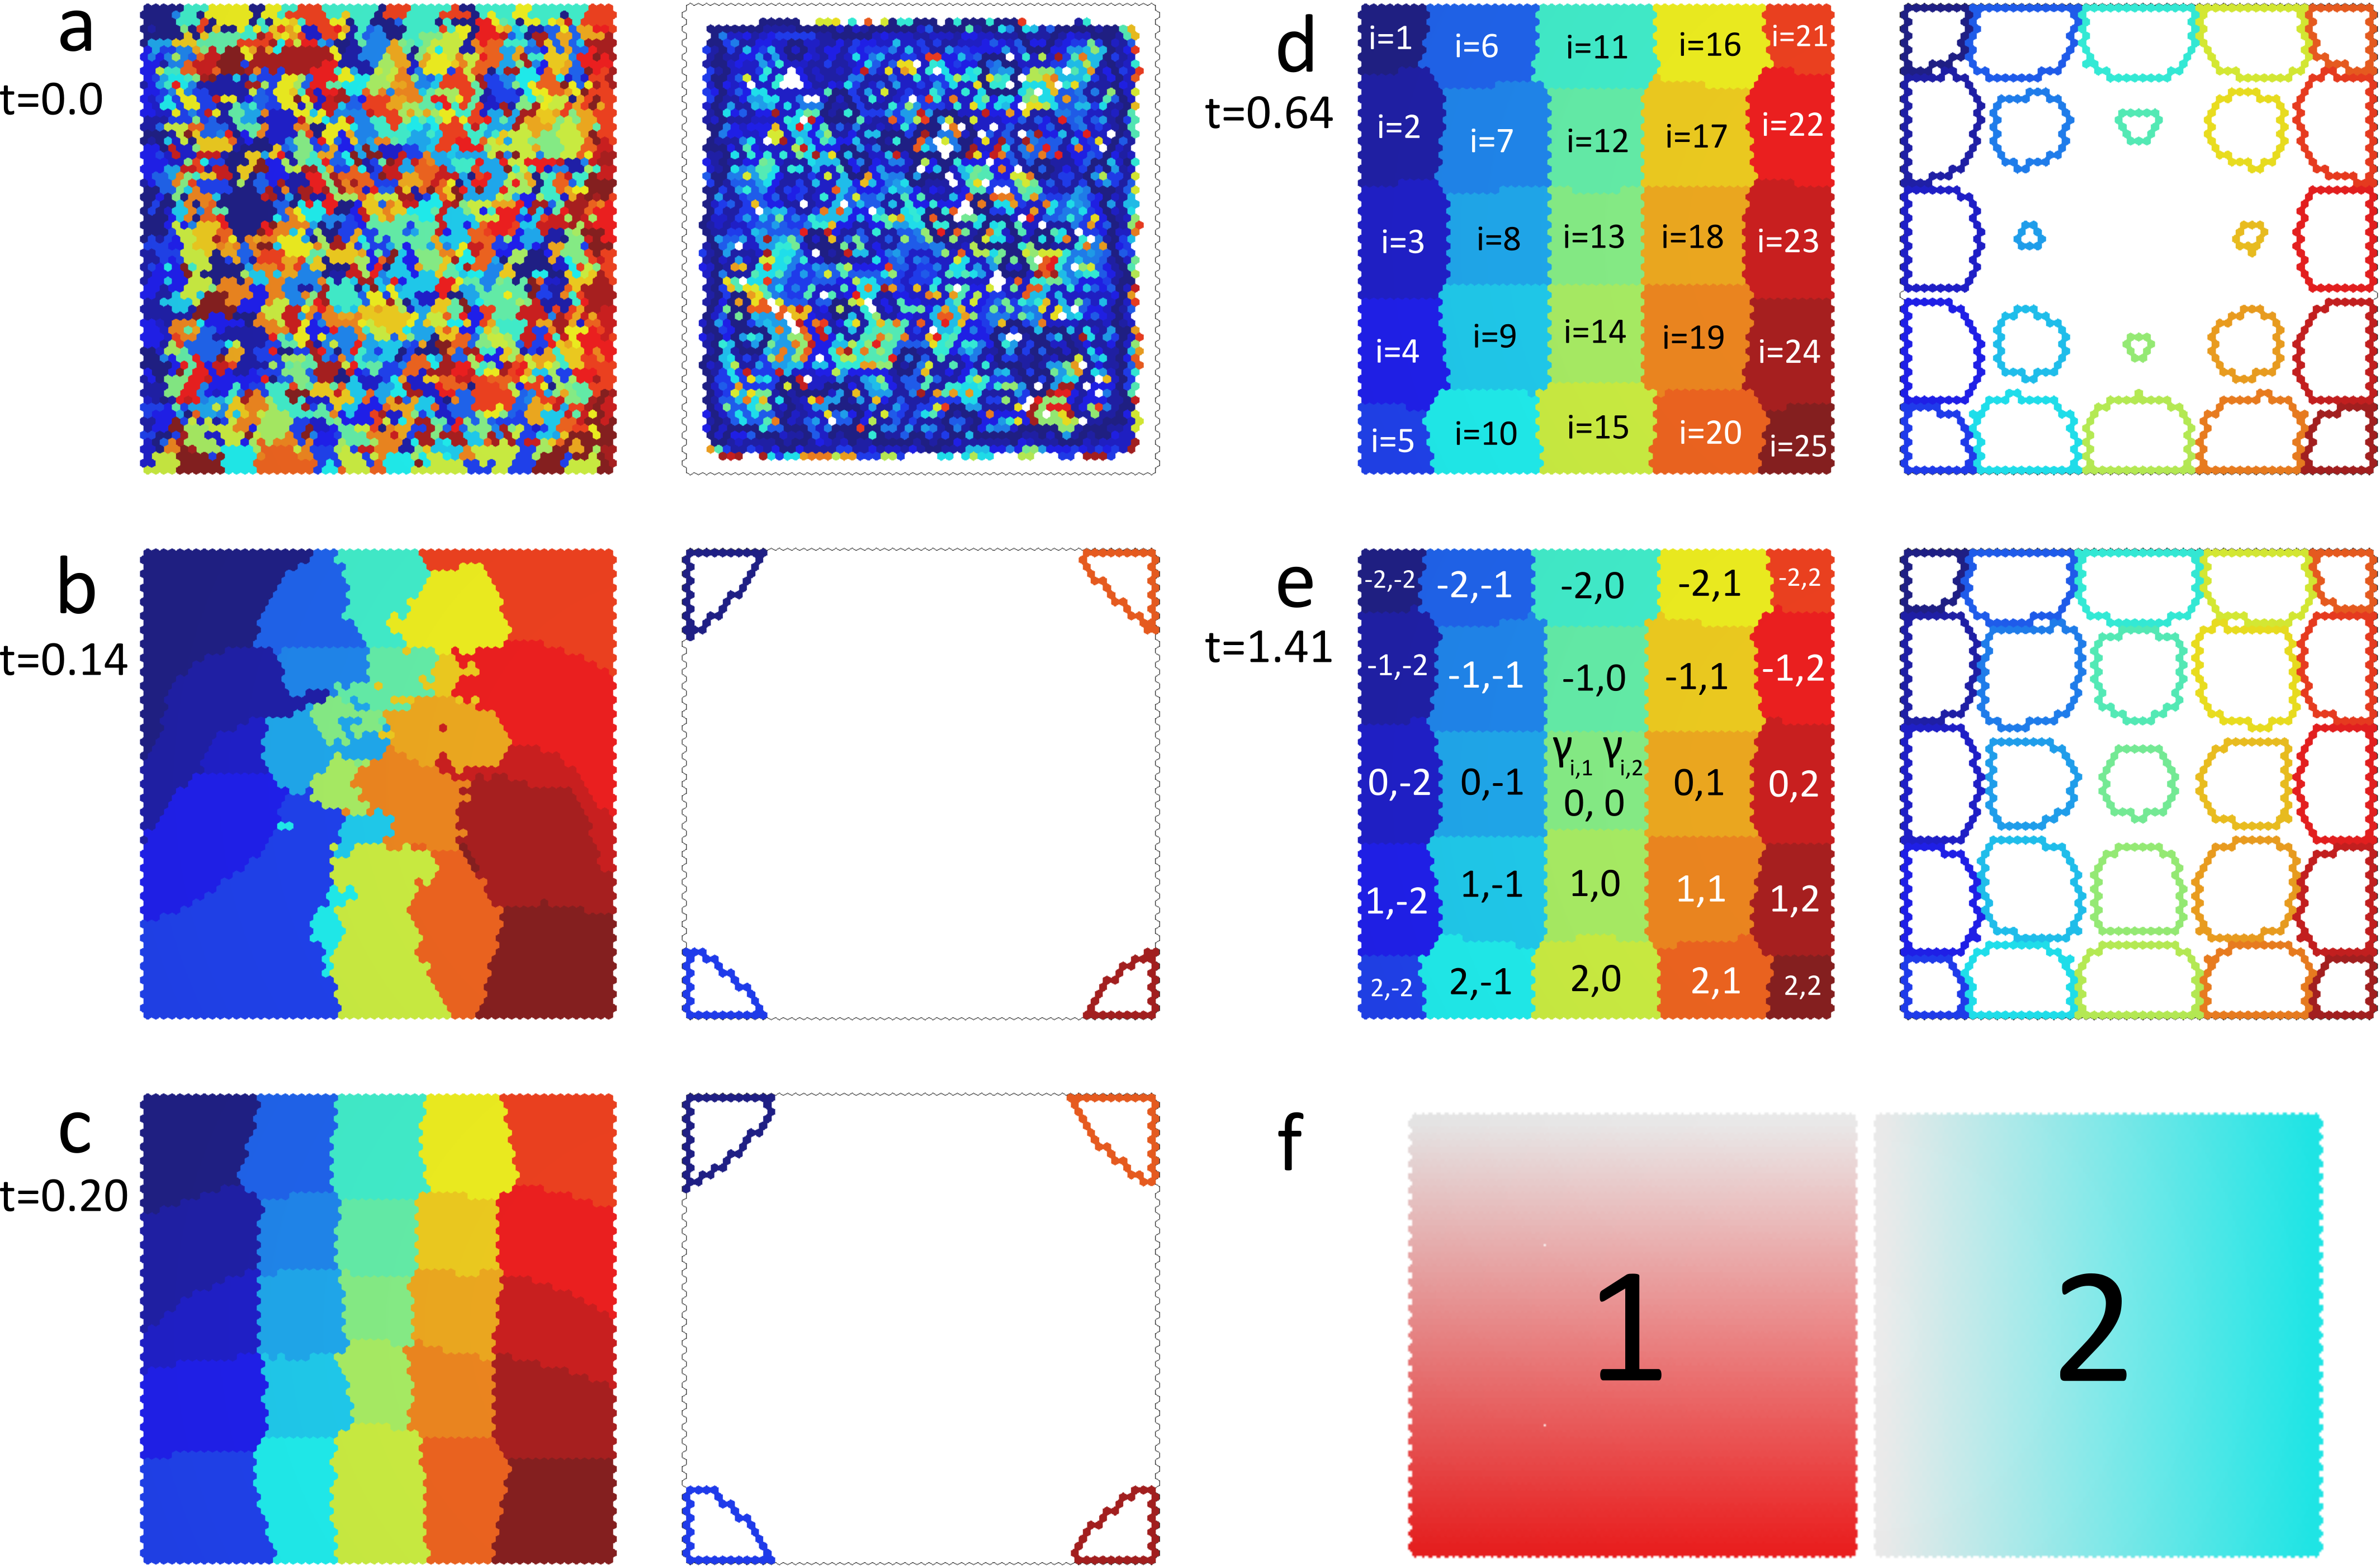
\includegraphics[width=\textwidth]{./Fig_25N2M_square/Fig_25N2M_square.png}
\end{center}
%\vspace{-0em}
\caption{\textbf{(a)--(e)} Connection densities of 25 thalamocortical axons
  simulated on a square domain. \textbf{(a)} Connection density at simulation
  time t=0. The left image shows a map of the identity of the thalamocortical
  axon type with the highest absolute connection density. Hexagonal elements
  coloured the darkest blue have the highest connection density for TC type
  $i=1$; those coloured the darkest red have maximal connection density in TC
  type $i=25$. The right hand image of each pair shows the hexes for which the
  connection density passes 0.5 for each TC type, giving a contour map. At
  t=0, connection densities are randomly distributed. \textbf{(b)} t=0.14. The
  grid-like organisation of the TC connections is beginning to emerge.
  \textbf{(c)} t=0.2. The 5x5 grid is now clear in the left map. Branching
  competition and differential interaction with the two guidance gradients is
  causing the branching, and therefore the connection densities, to localise in
  25 different locations. \textbf{(d)} t=0.64. Connection densities for each
  TC type have increased sufficiently for the contours to form. In (d), the
  mapping between colour and TC type $i$ is indicated. \textbf{(e)}
  t=1.41. Contours are well formed. In (e), the $\gamma$ values for each TC
  type, $i$, are shown. $\gamma_{i,1}$ gives the interaction with molecule `1'
  [red map in (f)]; $\gamma_{i,2}$ is the interaction with molecule
  `2'. \textbf{(f)} The two guidance gradients (`1' and `2') for this
  simulation.}
\label{fig:square}
\end{figure*}

\subsection*{The model can transfer realistic barrel patterns}

In which we show that a realistic barrel pattern in the thalamus can be
recreated in barrel cortex.

\subsubsection*{Stronger branching competition}

\cmnt{The realistic barrel pattern experiment is enhanced by stronger
  branching competition. This section may be required here or elsewhere.}

To increase the strength of the competition, we could take the power
of the branching density:
%
\begin{equation} \label{eq:branch_comp_pow}
\chi(\mb{x}, t) = - \frac{\epsilon  a_i}{N-1} \sum_{i' \ne i}^{N} (a_{i'})^l
\end{equation}
%
with $l>1$. This competition term can quickly become excessively large, so to
preserve the geometric shape of the function for small $a$, whilst
representing the idea that the amount of branching competition has an upper
bound, we pass the function through a logistic function.  This leads to the
following branching equation:

%
\begin{equation} \label{eq:branch_comp_pow_logistic}
\chi(\mb{x}, t) = - \frac{\epsilon a_i}{N-1} \sum_{i' \ne i}^{N}
\frac{1}{1 + e^{-m (a_{i'})^l}} - \frac{1}{2}
\end{equation}
%
$\epsilon$ represents the maximum value of the competition term for TC type
$i$. The parameters $l$ and $m$ control the steepness and shape of the
function.

%%% End of stronger branching competition %%%%%%%%%%%%%%%%%%%%%%%%%%%%%%%%%%%%

\begin{figure*}
\begin{center}
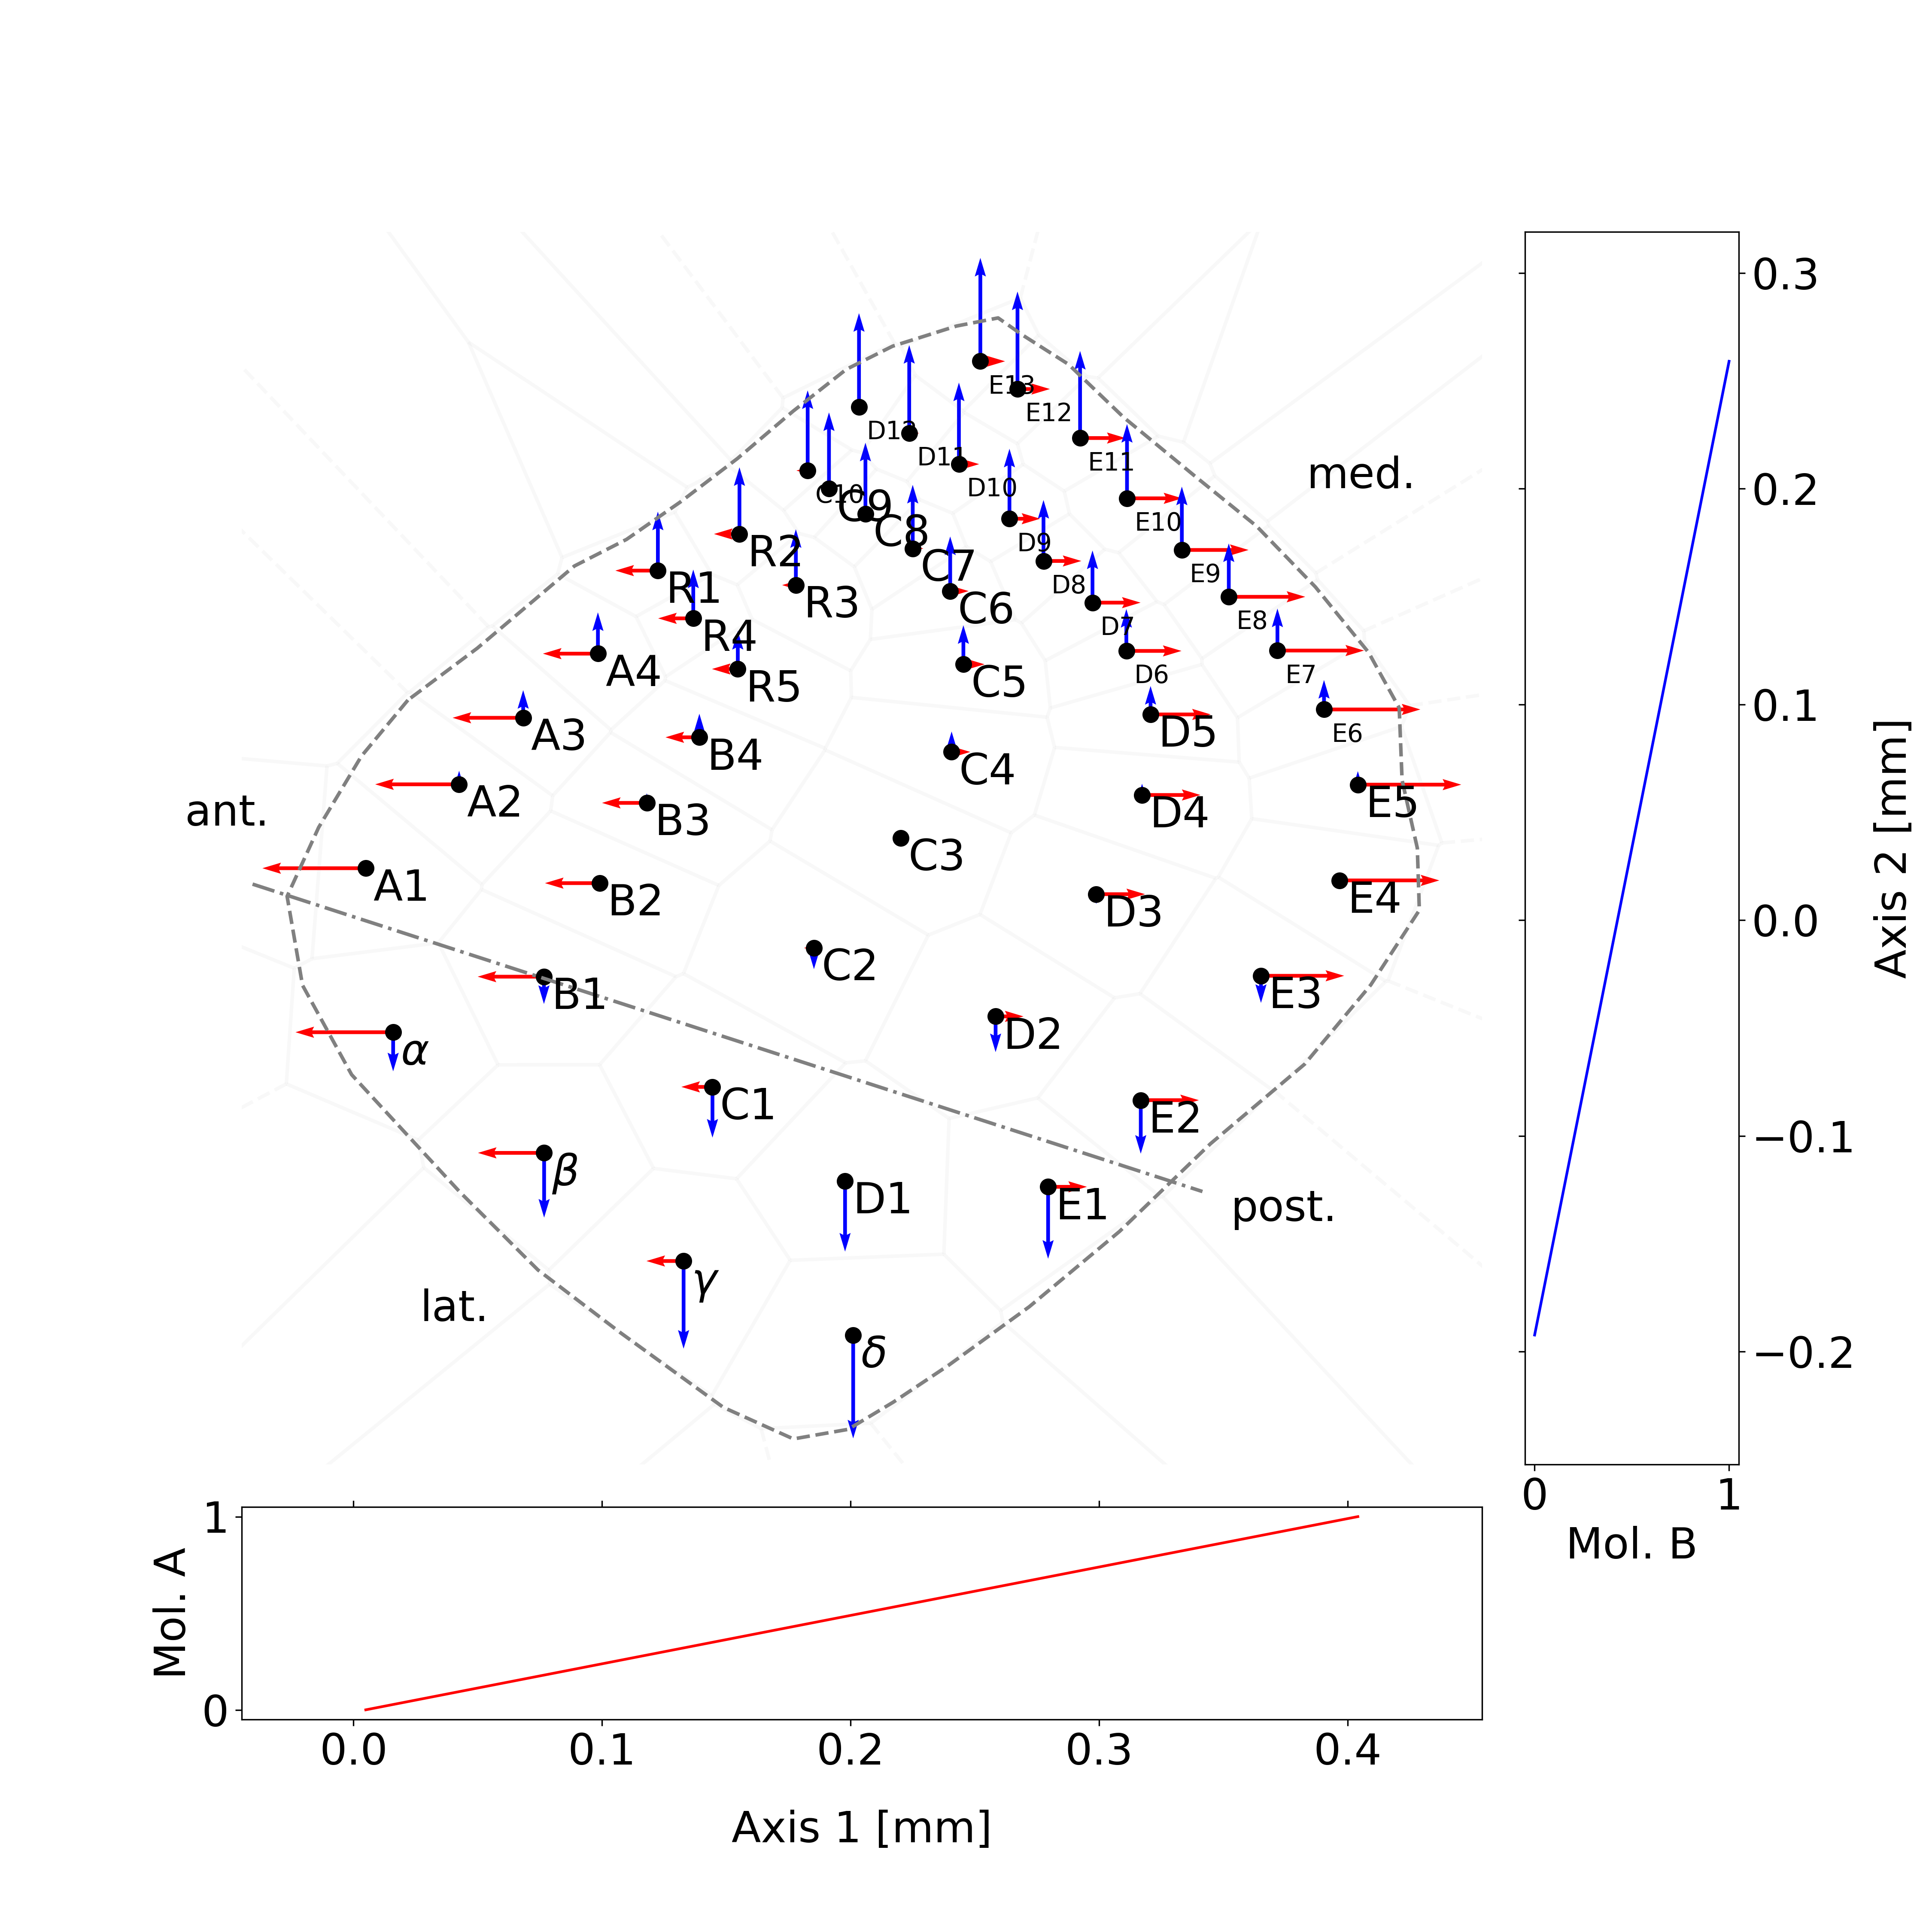
\includegraphics[width=0.7\textwidth]{../boundaries/barreloids_haidarliu_graph.png}
\end{center}
%\vspace{-0em}
\caption{Barreloid centres taken from \cite{haidarliu_size_2001} are shown as
  black circles. It is assumed that there are two linearly increasing,
  orthogonal signalling gradients (molecules A \& B) in the thalamus (side
  graphs), such that the location of each barreloid within the graded thalamic
  signal field can differentiate the efferent axons, with the result that
  axons from each barreloid interact to varying degrees with cortical
  signalling gradients. Coloured arrows show, for each barreloid, the
  magnitude (and sign) of the interaction that its thalamocortical projection
  will have with the signalling gradients in the cortex. The mappings from
  barreloid location to interaction strength are linear.}
\label{fig:barreloids}
\end{figure*}


\begin{figure*}
\begin{center}
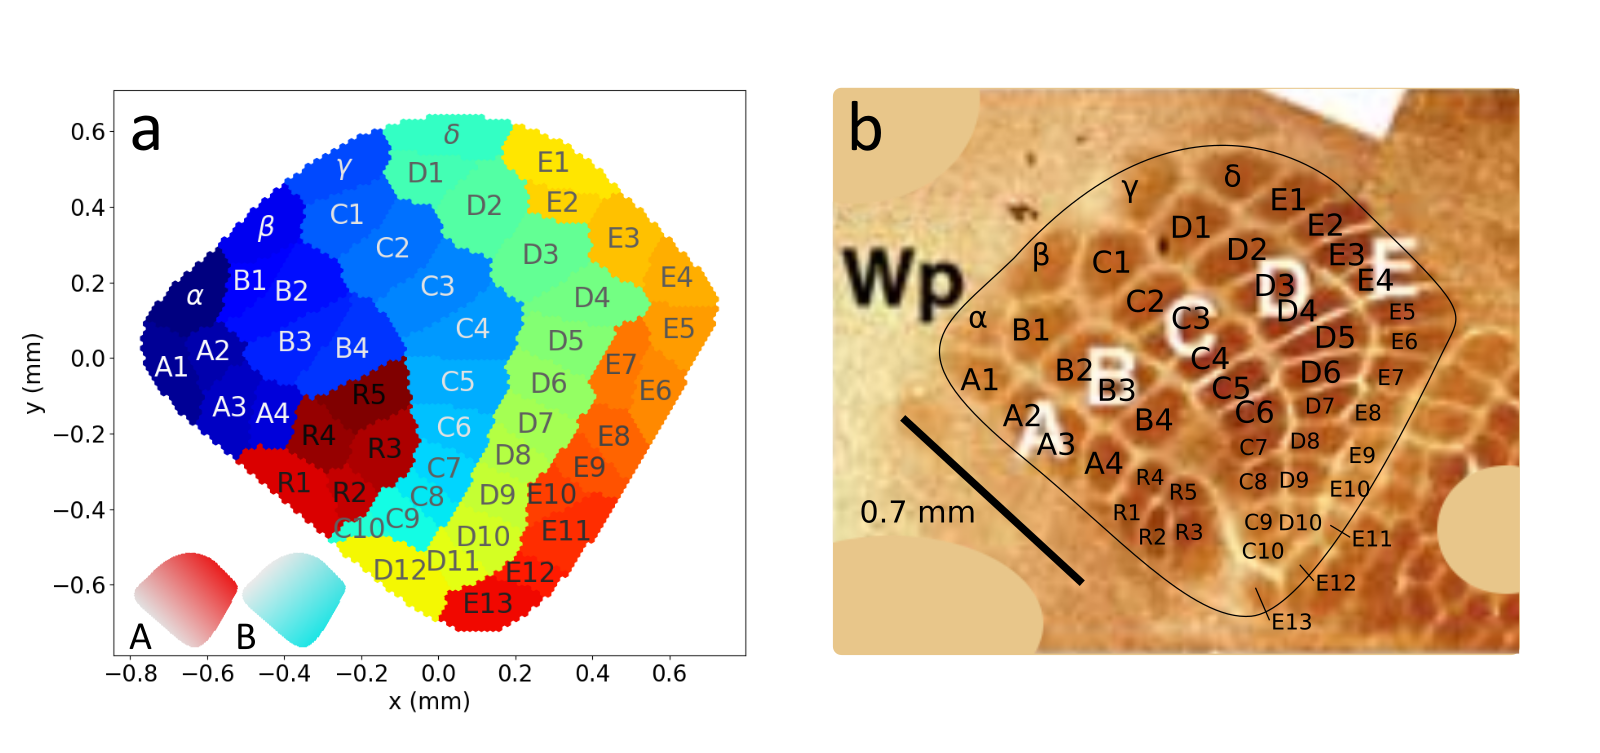
\includegraphics[width=\textwidth]{./realistic_barrels.png}
\end{center}
%\vspace{-0em}
\caption{Realistic barrel pattern}
\label{fig:barrels}
\end{figure*}


\subsection*{The barrel field reacts to changes in the expression pattern of guidance molecules}

To cover the reaction to changes in the guidance molecules caused by
experiments like those by Shimogori \& Grove.

Linear, circ linear, exponential, etc.

\subsection*{The barrel field reacts to simulated whisker plucking}

A section on whisker plucking?

%\subsubsection*{With surrounding large domains}
%Maybe, put this in to remind myself that I did this. It looks nice.

%\subsection*{Plucking experiments}
%Include results of plucking a single whisker, a row of whiskers and a
%column of whiskers.

%\subsection*{Any parameter sweeps necessary to show behaviour is
%  robust to changes in params}

\subsection*{Extending the model to capture row and arc development}

\subsubsection*{Manipulating Competition: Group competition stronger/weaker than inter-group competition}

Just an idea - have two separate epsilons.

\subsubsection*{Manipulating Guidance: Relative interaction strengths}

One possibility is to modify the strength of the guidance interactions of the
two, orthogonal guidance gradients. In the simulation we modify the magnitude
of the expression of each guidance molecule, although this is equivalent to,
and could stand for a more or less vigourous movement of axons in response to
un-modified guidance gradients.

\subsubsection*{Manipulating Guidance: Delayed onset in one axis}

Another idea; begin with only one guidance gradient, or one strong and
one very weak guidance gradient, and begin the development in this
form, so as to encourage the formation of rows. Subsequently, turn on
the second strong guidance signal.


%\begin{equation}
%\chi=\frac{\epsilon_i  a_i}{N-1} \sum_{j \ne i}^{N} a_j(\mb{x}, t)^l
%\end{equation}

%And normalization step

%\begin{equation}\label{eq:norm_comp8}
%a_i' = n_e \; \frac {a_i} {\textstyle \sum_j^{n_e} a_{i,j} }
%\end{equation}

%($a_i'$ becomes $a_i$ in the next computational step.)

\section*{Discussion}

We set out to test the hypothesis that barrel patterning may emerge via
self-organising processes. We first extended an existing model of neocortical
arealization to simulate pattern formation in two dimensions, inheriting from
this model the assumption that axonal branching and synaptogenesis are
coupled, and that thalamic projections compete for cortical territory under
the influence of molecular signalling gradients. Realistic barrel patterning
emerged only when terms were added to represent the assumption that
thalamocortical projections compete for a limited supply of connections with
cortical cells, that their branching rates are reduced by the branching of
other thalamocortical projections, and that the density of axon branching is
conserved for each projection. The net effect of these local interactions is a
Voronoi tesselation in which localised clusters of thalamic projections become
somatotopically organised on the cortical sheet according to the relative
values of coefficients specifying the rates at which axons are attracted and
repelled by orthogonal pairs of molecular signal gradients. According to this
model, the pattern of barrels is determined by the competitive and cooperative
interactions between cells relative to the shape of the cortical field
boundary. In simulation, we systematically investigated the origin of the
asymmetry between the barrel rows and arcs, and identified {\color{red} XXXXX}
as the most likely candidate for the elongation of barrel shapes along the
rows.

\bibliography{BarrelEmerge}

\end{document}


%%%%% ORIGINAL EQUATIONS MAINTAINED AS NOTES HERE FOR REFERENCE

\section*{App 1: Karbowski system with N TCs and M gradients}
%
\begin{equation} \label{eq:Karb2D_dc}
\frac{\partial c_i(\mb{x},t)}{\partial t} = -\alpha c_i(\mb{x},t) + \beta n(\mb{x},t)
[a_i(\mb{x},t)]^k
\end{equation}
%
\begin{equation} \label{eq:Karb2D_conserve}
n(\mb{x},t) = 1 - \sum_{i=1}^{N} c_i(\mb{x}, t)
\end{equation}
%
\begin{equation} \label{eq:Karb2D_da}
\frac{\partial a_i(\mb{x},t)}{\partial t}
= \nabla\vcdot\mb{J}_i(\mb{x},t) - \frac{\partial c_i(\mb{x},t)}{\partial t}
\end{equation}

with the flux current

\begin{equation} \label{eq:Karb2D_J}
\mb{J}_i(\mb{x},t) = D \nabla a_i(\mb{x},t) - a_i
\sum_{j=1}^M \big(\gamma_{i,j} \nabla\rho_j(\mb{x}) \big)
\end{equation}

The boundary condition applied to these equations is:

\begin{equation}
\mb{J}_i(\mb{x},t) \bigg\rvert_{boundary} = 0
\end{equation}

\section{App 2: Karbowski system with N TCs and M gradients plus competition}

%
\begin{equation} \label{eq:dc2}
\frac{\partial c_i(\mb{x},t)}{\partial t} = -\alpha c_i(\mb{x},t) + \beta n(\mb{x},t)
[a_i(\mb{x},t)]^k
\end{equation}
%
\begin{equation} \label{eq:conserve}
n(\mb{x},t) = 1 - \sum_{i=1}^{N} c_i(\mb{x}, t)
\end{equation}
%
\begin{equation} \label{eq:da2}
\frac{\partial a_i(\mb{x},t)}{\partial t}
= \nabla\vcdot\mb{J}_i(\mb{x},t) - \frac{\partial c_i(\mb{x},t)}{\partial t}- \frac{\epsilon_i  a_i}{N-1} \sum_{j \ne i}^{N} a_j(\mb{x}, t)^l
\end{equation}

And normalization step

\begin{equation}\label{eq:norm_comp8}
a_i' = n_e \; \frac {a_i} {\textstyle \sum_j^{n_e} a_{i,j} }
\end{equation}

($a_i'$ becomes $a_i$ in the next computational step.)
